\textbf{Результаты работы.}
\begin{enumerate}
	\item \textit{Представить разностный аналог краевого условия при $x = l$
	и его краткий вывод интегро-интерполяционным методом.}  
	
	Проинтегрируем (\ref{formula1}) на отрезке $[x_{N-1/2}; x_{N}]$:
	\begin{align*}
		\int_{x_{N-1/2}}^{x_{N}} dx \int_{t_m}^{t_{m+1}} c(T) \frac{\partial T}{\partial t} dt 
		=	
		- \int_{t_m}^{t_{m+1}} dt \int_{x_{N-1/2}}^{x_{N}} \frac{\partial F}{\partial x} dx 	 
		- \\ -
		\int_{x_{N-1/2}}^{x_{N}} dx \int_{t_m}^{t_{m+1}} p(x)T dt 
		+
		\int_{x_{N-1/2}}^{x_{N}} dx \int_{t_m}^{t_{m+1}} f(x)dt
	\end{align*}
	
	Пользуясь методами приближённого интегрирования получаем:
	\begin{align*}
		\frac{h}{4}\big(\hat{c}_N (\hat{T}_N - T_N) + \hat{c}_{N-1/2} (\hat{T}_{N-1/2} - T_{N-1/2})\big)
		=
		- \tau(\hat{F}_{N} - \hat{F}_{N-1/2})
		- \\ -
		\tau \frac{h}{4}(p_{N}\hat{T}_{N} + p_{N-1/2}\hat{T}_{N-1/2})
		+
		\tau \frac{h}{4}(\hat{f}_{N} + \hat{f}_{N-1/2})
	\end{align*}
	
	Учитывая краевые условия:
	\begin{multline*}
		\frac{h}{4}\big(\hat{c}_N (\hat{T}_N - T_N) + \hat{c}_{N-1/2} (\hat{T}_{N-1/2} - T_{N-1/2})\big)
		= \\
		- \tau(\alpha_N(\hat{T}_N - T_0) - \hat{\chi}_{N-1/2} \dfrac{\hat{T}_{N-1} - \hat{T}_{N}}{h})
		- \\ -
		\tau \frac{h}{4} (p_{N}\hat{T}_{N} + p_{N-1/2}\hat{T}_{N-1/2})
		+
		\tau \frac{h}{4} (\hat{f}_{N} + \hat{f}_{N-1/2})
	\end{multline*}
	
	
	Приводим к форме $\hat{K}_N \hat{T}_{N} + \hat{M}_{N-1} \hat{T}_{N-1} = \hat{P}_N$.
	\begin{equation*}
		\begin{cases}
			K_N = \dfrac{h}{8}(2\hat{c}_N + \hat{c}_{N-1/2}) + \dfrac{h\tau}{8}(2p_N + p_{N-1/2}) + \tau(\alpha_N - \dfrac{\hat{\chi}_{N-1/2}}{h}) \\
			M_N = \dfrac{h}{8}\hat{c}_{N-1/2} + \dfrac{h\tau}{8}p_{N-1/2} - \tau\dfrac{\hat{\chi}_{N-1/2}}{h} \\ 
			P_N = \dfrac{h}{4}(\hat{c}_N T_N + \hat{c}_{N-1/2} \dfrac{T_N + T_{N-1}}{2}) + \dfrac{h \tau}{4} (\hat{f}_{N} + \hat{f}_{N-1/2}) +  \tau \alpha_N T0\\
		\end{cases}
	\end{equation*}
	

	
	\newpage
	\item \textit{График зависимости температуры T(x, $t_m$) от координаты x при фиксированных значениях времени $t_m$ при заданных выше параметрах.}\\
	
	$\tau = 0.01$, $\varepsilon = 10^{-5}$
	
	\begin{figure}[h]
		\begin{center}
			{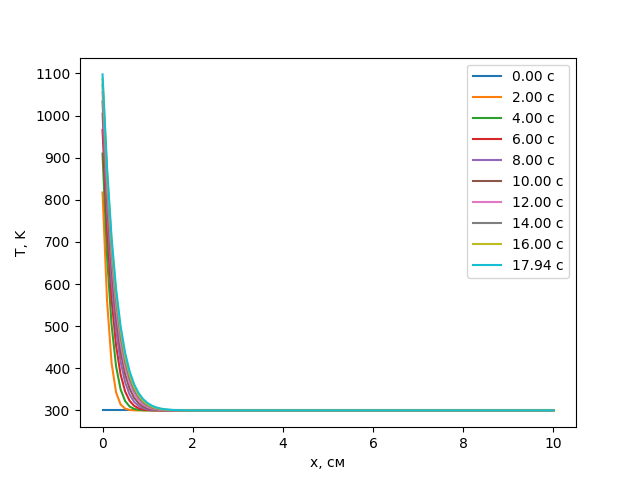
\includegraphics{../pictures/Figure_1}}
			\caption{Задание 2}
		\end{center}
	\end{figure}

	\item\textit{График зависимости $T(x_n, t)$ при нескольких значениях координаты $x_n$}
	\begin{figure}[h]
		\begin{center}
			{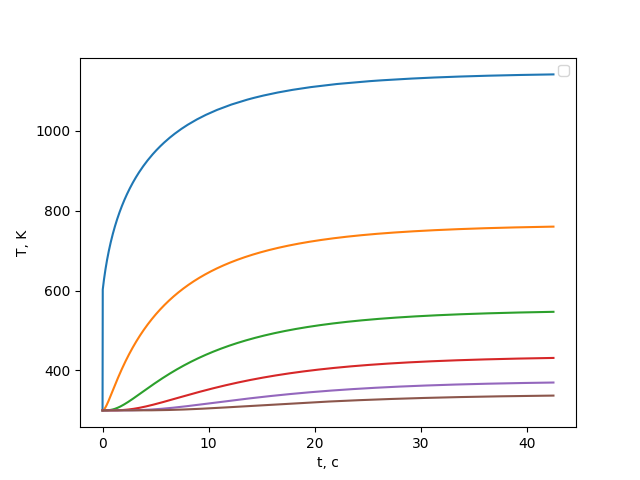
\includegraphics{../pictures/Figure_2}}
			\caption{Задание 3}
		\end{center}
	\end{figure}
	
\end{enumerate}